\documentclass[12pt,a4paper]{article}
\usepackage[utf8]{inputenc}
\usepackage[spanish]{babel}
\usepackage{amsmath}
\usepackage{amsfonts}
\usepackage{amssymb}
\usepackage{imakeidx}
\usepackage{graphicx}
\usepackage{apacite}
\usepackage{xcolor}
\setlength{\parindent}{0pt}
\addto\captionsspanish{% Replace "english" with the language you use
  \renewcommand{\contentsname}%
    {Tabla de contenidos}%
}
\usepackage[left=2.54cm,right=2.54cm,top=2.54cm,bottom=2.54cm]{geometry}
\author{Antonio Morán Muñoz}
\title{Caso Práctico 1}
\usepackage{fancyhdr}
\pagestyle{fancy}
\lhead{CASO PRÁCTICO 1}
\rhead{\thepage}
\cfoot{Computadores Avanzados}
\renewcommand{\headrulewidth}{0.4pt}
\renewcommand{\footrulewidth}{0.4pt}
\begin{document}

\begin{titlepage}
\thispagestyle{empty}
\centering
	
\includegraphics[width=0.35\textwidth]{castilla.png}\par\vspace{1cm}
	{\scshape\LARGE Universidad de Castilla-La Mancha \par}
	\vspace{1cm}
	{\scshape\Large Computadores Avanzados\par}
	\vspace{1.5cm}
	{\huge\bfseries CASO PRÁCTICO 1\par}
	\vspace{2cm}
	{\Large\itshape Antonio Morán Muñoz\par}

	\vfill

% Bottom of the page
	{CURSO ACADÉMICO 2018/2019}
	\vfill
	{\large \today\par}
\end{titlepage}

\thispagestyle{empty}
\tableofcontents
\newpage

\section{Descripción}
Considera un SMP que usa un protocolo de coherencia de invalidación basado en bus. Cada procesador en el sistema es idéntico, y la siguiente información se aplica a cada procesador. El 50\% de las instrucciones ejecutadas por cada procesador son cargas o almacenamientos (las instrucciones son de 32 bits). De ellas, en media, el 70\% son lecturas a datos privados, el 20\% son escrituras a datos privados, el 8\% son lecturas a datos compartidos y el 2\% son escrituras a datos compartidos.\\

Cada procesador tiene una cache separada de primer nivel. La cache de instrucciones es de 16 KB, asociativa de dos vías y tiene bloques de 16 bytes. La cache de datos es de 16 Kbytes, correspondencia directa y bloques de 16 bytes. Las tasas de acierto en las caches son las siguientes: 97\% para datos privados, 95\% para datos compartidos y 98,5\% para instrucciones. El tiempo de acierto en cache es de un ciclo para ambas caches.\\

El bus del SMP tiene líneas separadas para direcciones y datos, 64 para datos y 32 para direcciones. El bus es atómico (no divide transacciones), tal que los buses de direcciones y datos pueden ser tratados como un único bus desde el punto de vista de la negociación. El bus funciona a la mitad de frecuencia que el procesador. Para lecturas, la memoria responde a peticiones de datos 12 ciclos después de habérsele presentado la dirección, y soporta un bloque de datos por ciclo de bus después de ello. Para escrituras, las direcciones y los datos son presentados a la memoria al mismo tiempo. Así, la escritura de una palabra consume un ciclo de bus, y la escritura de 16 bytes consume dos ciclos. Considera que todas las peticiones son satisfechas por el sistema de memoria y no por otras caches. El CPI es 2 sin considerar penalidades en el sistema de memoria.\\

\begin{center}
	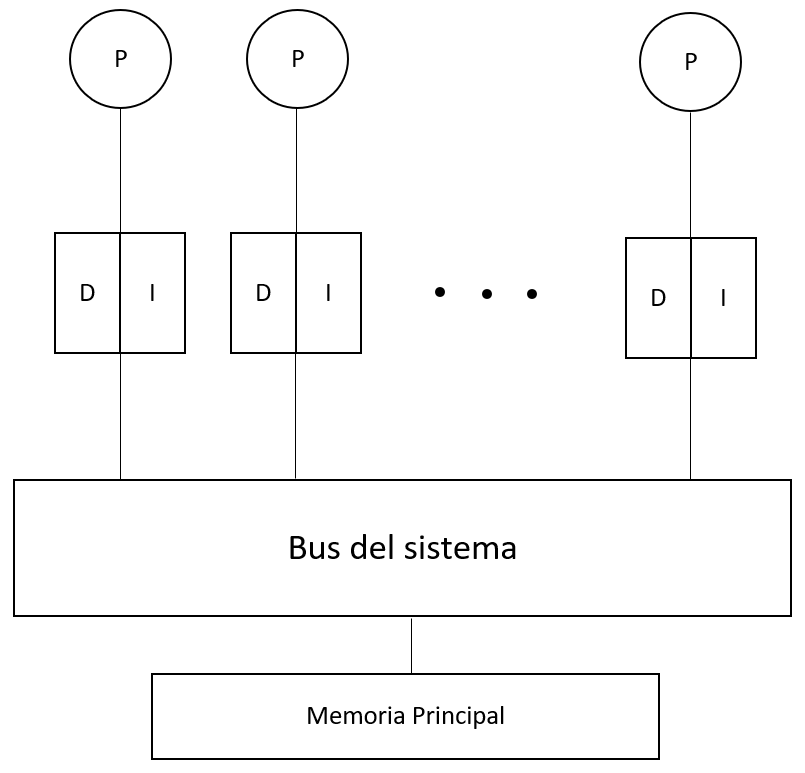
\includegraphics[width=0.6\textwidth]{diagrama.png}\par
\end{center}


\subsection{Apartado a)}

¿Cuál es la utilización que hace del bus un único procesador si las caches usan políticas de escritura inmediata y carga en escritura? ¿Cuántos procesadores puede soportar el bus sin llegar a saturarse?\\

Ignora la contención en el bus y los mensajes de coherencia recibidos desde otros procesadores, pero considera el tráfico debido al protocolo de coherencia generado por el procesador. 

\subsubsection{Solución}
Para responder a la primera cuestión, primero tendremos que aplicar la siguiente fórmula.
\begin{equation}
\text{Uso}=\frac{CPI_{extra}}{CPI_{total}}
\end{equation}

Donde $CPI_{extra}$ son los CPI que emplea en el bus el procesador, y $CPI_{total}$ es el $CPI_{ideal}$ (que es el CPI si no se usara nunca el bus) más el $CPI_{extra}$. Por lo tanto, nuestra primera misión será calcular el $CPI_{extra}$ que requiere un procesador, que será debido principalmente a fallos en la caché, escrituras, políticas de escritura...\\

Para calcular el $CPI_{extra}$, tenemos que calcular por un lado el $CPI_{datos}$ y, por otro, el $CPI_{instrucciones}$. De tal manera que dicho $CPI$ total sería la suma de ambos:
\begin{equation}
CPI_{total}=CPI_{datos}+CPI_{instrucciones}
\end{equation}

Por otro lado, los datos se dividen en dos categorías: privados y compartidos. Por lo tanto, $CPI_{datos}$ lo podemos dividir en $CPI_{privados}$ y $CPI_{compartidos}$:
\begin{equation}
CPI_{datos}=CPI_{privados}+CPI_{compartidos}
\end{equation}

Pero todavía no hemos acabado, tanto el acceso a datos privados como a compartidos se puede dividir en otras dos categorías: lectura o escritura. Por tanto, tendremos que distinguir entre los accesos que son de escritura y los de lectura, ya que nos darán un CPI diferente:
\begin{align}
CPI_{privados}=CPI_{lec.priv}+CPI_{esc.priv}\\
CPI_{compartidos}=CPI_{lec.com}+CPI_{esc.com}
\end{align}

A continuación, vamos a calcular las diferentes expresiones desde dentro hacia fuera. Empecemos por los datos privados. Para la lectura, tenemos que ver cuántos ciclos llevaría leer en caso de fallo en caché (en caso de acierto, se tarda 1 ciclo, que ya se incluye dentro del $CPI_{ideal}$). En caso de fallo, tendríamos que ir hacia memoria principal. En primer lugar tenemos que llevar la dirección del dato que queremos leer, lo que consume un ciclo de bus (que es igual que dos ciclos de procesador). Una vez que tenemos la dirección en memoria, el enunciado nos dice que ésta tarda 12 ciclos de bus (6 de procesador) en responder y, un ciclo de bus (0.5 de procesador) extra por bloque de datos. Como un bloque de datos tiene 16B, pero el bus de datos solo puede transportar 8B, tenemos que usar 2 (4) ciclos para mover un bloque. Una vez que hemos traído el bloque a caché, se tarda un ciclo de procesador en llevarlo de cache al procesador (ciclo que no tenemos en cuenta en los cálculos porque se incluye en el $CPI_{ideal}$). Por lo tanto, tenemos que cada fallo de lectura de datos supone un extra de $2+24+8=34$ ciclos. Como la probabilidad de que se produzca un fallo de este tipo es e $1-0.97=0.03$, tenemos que multiplicar los ciclos por esta probabilidad. Además, hay que tener en cuenta que el porcentaje de cargas/almacenamientos es del 50\%, del cual el 70\% son de lectura a datos privados. En consecuencia, tenemos que ponderar lo anterior por $0.5\cdot 0.7=0.35$, que será el porcentaje de instrucciones de este tipo que se ejecuten en el procesador. Resumiendo todo lo anterior en una ecuación, quedaría lo siguiente:
\begin{align*}
CPI_{lec.priv}&=0.35\cdot (0.03\cdot (34))=0.357\text{ CPI}
\end{align*}

En cuanto a la escritura de datos privados, hay que tener en cuenta que tenemos una política de escritura inmediata y carga en escritura (una combinación que no es muy usual). Por lo tanto, cada vez que ocurra un fallo, habrá que leer de memoria el bloque que se quiere escribir y traerlo a caché. Una vez que se haya hecho esto, habrá que escribir tanto en caché como en memoria principal dicho bloque (por la escritura inmediata). A continuación, describiremos la secuencia de acontecimientos: cuando ocurre un fallo en cache, tenemos que traer el bloque que queremos escribir a caché, como hemos dicho anteriormente. Esto requiere 34 ciclos, que ya calculamos previamente cuando analizamos la lectura de datos privados. Una vez leído el bloque, toca escribir en caché y en memoria (\textit{escritura inmediate}). La escritura en caché lleva 1 ciclo de procesador. Tras esto, toca contar los ciclos que se tarda en escribir en memoria. El procesador enviará por el bus la dirección del bloque que se quiere escribir y el bloque (hay que recordar que la comunicación con memoria principal es a nivel de bloque). Como dicho bloque tiene un tamaño de 16B, pero el bus de datos tiene capacidad para 8B, se requieren dos (4) ciclos para llevar todo el bloque a memoria y escribirlo. Y ya está, según el enunciado no parece haber ninguna otra penalización en el proceso de escritura. Resumiendo, para la escritura de datos privados en caso de fallo tenemos una penalización de $34+1+4=39$ ciclos. Por último, y al igual que en el caso anterior, tenemos que ponderar los ciclos por la tasa de fallo y por el porcentaje de dicha instrucción en el global (dichos valores se muestran directamente en la ecuación). La ecuación que resulta de todo lo anterior sería la siguiente:
\begin{align*}
CPI_{esc.priv}&=0.1\cdot (0.03\cdot (39))=0.117\text{ CPI}
\end{align*}

Sustituyendo los valores recién obtenidos en $(3)$, tenemos:
\begin{align*}
CPI_{privados}=0.357+0.117=0.474 \text{ CPI}
\end{align*}

El siguiente paso es repetir el proceso anterior, pero con los datos compartidos. La lectura de este tipo de datos no tiene mucha complicación, ya que, según el enunciado, se lleva a cabo siempre desde memoria principal. Por lo tanto, se tardará el mismo número de ciclos que cuando se leen datos privados, es decir, 34. Tomando los porcentajes correspondientes que se nos dan en el enunciado, nos queda la siguiente ecuación:
\begin{align*}
CPI_{lec.com}&=0.04\cdot (0.05\cdot (34))=0.068\text{ CPI}
\end{align*}

En cuanto a la escritura de datos compartidos, tenemos que tener el tráfico generado por el protocolo de coherencia. Como la estrategia de escritura es \textbf{escritura inmediata} y \textit{carga en escritura}, la ecuación no cambiará en ese apartado. No obstante, cada vez que se escriba algo que es compartido por otros procesadores, hay que escribirlo en la caché de éstos. Como hay que actualizar un bloque, éste tardará dos ciclos de bus (4 de procesador) en llevarlo al resto de cachés. En consecuencia, a los ciclos que ya teníamos (multiplicado por la tasa de fallos) habrá que sumarle estos cuatro ciclos y multiplicarlo todo por el porcentaje global de este tipo de instrucciones:
\begin{align*}
CPI_{esc.com}&=0.01\cdot (0.05\cdot (39)+4)=0.0595\text{ CPI}
\end{align*}

Sustituyendo estos valores en $(4)$, tenemos:
\begin{align*}
CPI_{compartidos}=0.068+0.0595=0.1275 \text{ CPI}
\end{align*}

Ahora, podemos sustituir en $(2)$:
\begin{equation*}
CPI_{datos}=0.474+0.1275=0.6015\text{ CPI}
\end{equation*}

Por último, sólo queda calcular $CPI_{instrucciones}$. En caso de que no se encuentre la instrucción en la caché correspondiente, se tendrá que buscar en la memoria principal, igual que hacíamos cuando leíamos un dato. Esto podría hacernos pensar que el número de ciclos que esto requiere es igual que en esos casos. Sin embargo, como las instrucciones son de 32 bits y el bus de direcciones soporta esos 32 bits, no será necesario hacer dos veces el camino para traer la dirección completa. En consecuencia, sólo se consume un ciclo de bus (2 de procesador) para traer una instrucción (más los 12 que tarda la memoria en responder):
\begin{align*}
CPI_{instrucciones}=0.015\cdot (24+2)=0.39 \text{ CPI}
\end{align*}

Teniendo este dato, ya podemos sustituir en $(1)$:
\begin{equation*}
CPI_{extra}=0.6015+0.39=0.9915\text{ CPI}
\end{equation*}

A continuación, tenemos que sumar este resultado al $CPI_{ideal}$ para conocer el $CPI_{total}$:
\begin{equation*}
CPI_{total}=CPI_{ideal}+CPI_{extra}=2+0.9915=2.9915\text{ CPI}
\end{equation*}

Una vez conocidos $CPI_{total}$ y $CPI_{extra}$, sólo resta hacer una división para conocer el uso que hace el procesador del bus:
\begin{align*}
\text{Uso}&=\frac{CPI_{extra}}{CPI_{total}}\\
\text{Uso}&=\frac{0.9915}{2.9915} = 0.331 = 33.1\%
\end{align*}

Ahora, vamos a contestar a la segunda pregunta. Para que el bus se sature, su uso debe alcanzar el $100\%$ por parte de todos los procesadores que trabajen sobre él. Por lo tanto, si un sólo procesador hace un uso del $33.1\%$, con cuatro procesadores ya estaríamos superando ese umbral, ya que $33.1\cdot 4=132.4\%$. En consecuencia, sólo podríamos conectar 3 procesadores ($33.1\cdot 3=99.3\%$) sin que se sature el bus. 

\subsection{Apartado b)}
¿Cuántos procesadores puede soportar el bus sin saturarse si las caches son de postescritura y carga en escritura? La probabilidad de tener que reemplazar un bloque modificado en la cache es de 0,3. \\

Ignora la contención en el bus y los mensajes de coherencia recibidos desde otros procesadores, pero considera el tráfico de coherencia generado por el procesador. Considera que un acierto en escritura a un bloque compartido genera sólo una transacción de invalidación, suponiendo un ciclo de bus. Considera que la postescritura no se solapa con la lectura de nuevos datos y que todos los aciertos de escritura a datos compartidos requieren la correspondiente transacción.

\subsubsection{Solución}

Para responder a la pregunta tenemos que repetir el procedimiento anterior, es decir, calcular el $CPI$ de cada cosa, después el uso que haría un solo procesador del bus y, por último, lo que nos piden. Pasemos, por tanto, a estudiar la lectura de datos privados:

Si un dato (privado o compartido) se encuentra en caché, no habrá penalización, ya que se tardaría un ciclo en pedir el dato y otro ciclo en mandarlo al procesador, que es igual a dos, lo que coincide con el $CPI_{ideal}$. Esto es así porque, según el enunciado, consideramos que las peticiones no son satisfechas por otras cachés. Es decir, suponemos que la caché local contiene la versión más actualizada del dato. En caso de fallo, tendríamos que tener en cuenta que existe una probabilidad del $30\%$ de reemplazar un bloque modificado. Como tenemos una política de \textit{postescritura}, cuando esto ocurra tendríamos que escribir el bloque modificado en memoria principal. En consecuencia, además de los 34 CPI extra que supone la lectura en memoria (lo hemos calculado en el primer apartado), hay que sumar los debidos a \textit{postescritura}. Como también demostramos en el primer apartado, llevar el bloque que se quiere escribir a memoria genera 4 ciclos (de procesador) adicionales, pues tenemos que llevar la mitad del bloque en un ciclo de bus y la otra mitad en el ciclo de bus siguiente. Por lo tanto, tendremos que añadir a nuestra ecuación este número de ciclos multiplicado por la probabilidad de que se reemplace un bloque modificado:
\begin{align*}
CPI_{lec.priv}&=0.35\cdot (0.03\cdot (34 + 0.3\cdot 4))=0.3696\text{ CPI}
\end{align*}

En cuanto a la escritura de datos privados, en caso de acierto no tenemos que escribir el bloque en memoria al mismo tiempo, por lo que en esta situación no utilizamos el bus y no supone una penalización. En caso de fallo, sin embargo, tenemos que traer el bloque de memoria a caché y escribirlo, debido a la política de \textit{carga en escritura}. Por lo tanto, se usará el bus para traer dicho bloque a caché y, en caso de que se reemplace por un bloque modificado, para escribir dicho bloque en memoria. En el apartado anterior vimos que leer un bloque de memoria a caché lleva 34 ciclos. Y acabamos de ver también que escribir un bloque modificado genera 4 ciclos. \textcolor{red}{Por último, tenemos que tener en cuenta el ciclo que requiere el escribir el bloque en caché, una vez que se ha traído de memoria}. Por lo tanto, la ecuación resultante sería la siguiente:
\begin{align*}
CPI_{esc.priv}&=0.1\cdot (0.03\cdot (34+0.3\cdot 4))=0.1056\text{ CPI}
\end{align*}

Sustituyendo los valores recién obtenidos en $(3)$, tenemos:
\begin{align*}
CPI_{privados}=0.3696+0.1056=0.4752 \text{ CPI}
\end{align*}

Pasemos ahora a estudiar los datos compartidos. Respecto a la lectura de los mismos, al igual que dijimos con los datos privados, no se generaría tráfico en el bus de memoria, ya que el enunciado nos dice que las lecturas de datos no son satisfechas por otras cachés (\textcolor{red}{¿Haría falta comprobar si el dato más reciente está en memoria?}). En caso de fallo, la situación también sería igual que con los datos privados, ya que llevaría 34 ciclos traer el dato de memoria y 4 ciclos escribir bloques modificados en la misma (con una probabilidad de 0.3 de que ocurra esto)(\textcolor{red}{¿Habría que actualizar en otras cachés en caso de que dicho bloque tenga datos compartidos?}).
\begin{align*}
CPI_{lec.com}&=0.04\cdot (0.05\cdot (34 + 0.3\cdot 4))=0.0704\text{ CPI}
\end{align*}

En cuanto a la escritura de datos compartidos, en caso de acierto, no bastará con escribir en caché solamente. También se genera una transacción de invalidación, que requiere dos ciclos de procesador (\textcolor{red}{¿Habría que tener en cuenta también el protocolo de coherencia?}). En caso de fallo, habría que traer el bloque de memoria y escribirlo. Leer un bloque de memoria conlleva 34 ciclos de procesador (el ciclo usado para escribir en caché no usa el bus, por lo que no lo tenemos en cuenta). La transacción de invalidación generaría dos ciclos de procesador más. También hay que tener en cuenta que se puede reemplazar un bloque que esté modificado, por lo que habría que escribirlo en memoria. Esto último, hemos visto que genera 4 ciclos extra. Por último, tenemos que contar los 4 ciclos de procesador debidos al protocolo de coherencia, que contarán tanto si hay fallos como si hay aciertos en caché. Condensando todo lo anterior en una ecuación, nos quedaría algo tal que así:
\begin{align*}
CPI_{esc.com}&=0.01\cdot (0.95\cdot (2) + 0.05\cdot (34+2+0.3\cdot 4)+4)=0.0776\text{ CPI}
\end{align*}

Sustituyendo estos valores en $(4)$, tenemos:
\begin{align*}
CPI_{compartidos}=0.0704+0.0776=0.148 \text{ CPI}
\end{align*}

Ahora, podemos sustituir en $(2)$:
\begin{equation*}
CPI_{datos}=0.4752+0.148=0.6232\text{ CPI}
\end{equation*}

En cuanto a las instrucciones, el razonamiento es exactamente igual que en el primer apartado, por lo que podemos usar directamente el resultado obtenido antes en $(1)$:
Teniendo este dato, ya podemos sustituir en $(1)$:
\begin{equation*}
CPI_{extra}=0.6232+0.39=1.0132\text{ CPI}
\end{equation*}

A continuación, tenemos que sumar este resultado al $CPI_{ideal}$ para conocer el $CPI_{total}$:
\begin{equation*}
CPI_{total}=CPI_{ideal}+CPI_{extra}=2+1.0132=3.0132\text{ CPI}
\end{equation*}

Una vez conocidos $CPI_{total}$ y $CPI_{extra}$, sólo queda hacer una división para conocer el uso que hace el procesador del bus:
\begin{align*}
\text{Uso}&=\frac{CPI_{extra}}{CPI_{total}}\\
\text{Uso}&=\frac{1.0132}{3.0132} = 0.331 = 33.6\%
\end{align*}

Con este porcentaje de uso por parte de un solo procesador, el bus se saturaría al poner 3, ya que $33.6\cdot 3=100.8\%$. Por lo tanto, con estas políticas habría que utilizar dos procesadores para aprovechar el bus al máximo sin que se llegue a saturar.

\bibliographystyle{apacite}
\bibliography{referencias}
\end{document}